\chapter{Konzeption}

Innerhalb dieses Kapitels werden verschiedene Teilbereiche dieser Masterarbeit erfasst und für jede Teilaufgabe ein Konzept erstellt.
Inhalt der Konzepte ist unter anderem die Definition der Aufgabe, sowie aller Komponenten, die zur Realisierung benötigt und verwendet werden.\\

An dieser Stelle wird das von der Universität zur Verfügung gestellte Emotiv EPOC als das \acs{BCI} für die späteren Tests der vorliegenden Arbeit definiert. \\


\section{Auswahl der BCI-Software}

Das Forschungsgebiet \acs{BCI} ist in den vergangenen Jahren immer umfangreicher geworden, so existieren mittlerweile eine ganze Reihe von Software Plattformen für die Arbeit mit \acs{BCI}s.
Die ausgewählte Software sollte möglichst alle nachfolgenden Kriterien erfüllen:

\begin{itemize}
\setlength{\itemsep}{0pt}
\footnotesize
{
\item Offener Quellcode
\item Nicht-kommerzielle Verwendung
\item Gute Dokumentation
\item Große und aktive Nutzergemeinschaft
\item Programmiersprache C++, C\# oder Java
\item Gute Software-Architektur für Erweiterungen oder Neuentwicklungen
\item Unterstützung des Emotiv EPOC und möglichst vieler anderer \acs{BCI}'s\\
}
\end{itemize}

Für diese Auswahl werden die \acs{BCI}-Software Plattformen BCI2000, OpenVibe, TOBI und BCI++ kurz vorgestellt, um darauf aufbauend die \acs{BCI}-Software für diese Masterarbeit auszuwählen.
Wichtig bei der Entscheidung ist die vorausgesetzte die Unterstützung des Emotiv EPOC Neuroheadset \cite{Emotiv2014}. \\


\subsubsection{BCI2000}
\acs{BCI2000} \cite{BCI2000Online} ist eine quelloffene Mehrzweckplattform für die Erforschung, Entwicklung und Verwendung von Brain Computer Interfaces. Sie ist in C++ geschrieben und in einer modularen Architektur aufgebaut. 
Sie unterstützt in der aktuellen Version das Betriebssystem Windows, zukünftig soll auch Linux und MacOS hinzugefügt.
Gegenwärtig werden 18 verschiedene Möglichkeiten der EEG-Datenakquirierung und viele Module zur Signalverarbeitung bereitgestellt. 
Darüberhinaus existiert eine umfangreiche Dokumentation für die Benutzung und Entwicklung von \acs{BCI2000}.\\


\subsubsection{BCI++}
BCI++ \cite{BCI++Online} ist ein in C++ entwickeltes Framework zur Erstellung prototypischer \acs{BCI}-Systeme und unterstützt eine Vielzahl an BCI- und Bio-Signal-Paradigmen. 
Der Aufbau des Frameworks ist in zwei Module unterteilt. Dem "`Hardware Interface Module"' (\acs{HIM}) und dem "`Graphical User Interface Module"' bezeichnet als \acs{AEnima}.
Das \acs{HIM} erhält und verarbeitet alle Signale und kommuniziert via TCP/IP mit \acs{AEnima}. 
\acs{AEnima} ermöglicht daraufhin die Realisierung der visuellen Präsentation unter Verwendung der Irrlicht 3D Engine \cite{IrrlichtOnline}. \\


\subsubsection{OpenVibe}
OpenVibe \cite{OpenVibeOnline} ist eine quelloffene in C++ entwickelte BCI-Software Plattform und wird regelmäßig vom \textit{"`French National Institute for Research in Computer Science and Control"'} aktualisiert. 
Sie ist auf das Erstellen, Testen und Benutzen von BCIs spezialisiert.
Zu diesem Zweck ermöglicht sie Nutzern ohne Programmierkenntnisse die Verwendung einer dazugehörigen Grafischen Benutzeroberfläche. 
OpenVibe verfügt über 15 verschiedene Möglichkeiten der EEG-Datenakquirierung (Stand: \today) und unterstützt die Betriebssysteme Windows und Linux.\\


\subsubsection{TOBI}
\ac{TOBI} ist ein europäisches Gemeinschaftsprojekt verschiedener Universitäten und medizinischer Einrichtungen \cite{TOBIOnline}.
Das Ziel ist die Entwicklung praktischer \acs{BCI}-Technologien. 
Es versucht in erster Linie die Interoperabilität zwischen unterschiedlichen \acs{BCI}'s zu erleichtern \cite{BCIPlatforms}.
Deshalb adres\-siert \acs{TOBI}, im Gegensatz zu den bereits vorgestellten BCI-Software Plattformen, insbesondere Entwickler, um die Kompatibilität zwischen anderen \acs{BCI}-Produkten oder -Komponenten zu verbessern.
Darüberhinaus versucht \acs{TOBI} die Standardisierung von BCIs zu erreichen.\\


Die Wahl der BCI-Software Plattform in dieser Arbeit fiel auf BCI2000.
Alle anderen hier vorgestellten Alternativen sind damit in keinster Weise als ungeeignet zu bezeichnen, da die Kriterien ebenfalls von fast allen erfüllt wurden.
Ausschlaggebend für die Entscheidung war daher hauptsächlich die modulare Architektur von BCI2000, 
da die Unterteilung in "`Source"'-, "`Signal-Processing"'- und "`User-Application"'-Modul sehr präzise den Einstiegspunkt dieser Arbeit abgrenzt.
Somit kann ein "`User-Application"'-Modul erstellt werden, während andere für diese Arbeit nicht relevanten Bereiche unangetastet bleiben.
Außerdem verfügt BCI2000 über eine sehr umfangreiche Dokumentation und findet häufig Verwendung in wissenschaftlichen Veröffentlichungen.
BCI2000 konnte zudem gegenüber OpenVibe mehr unterstützte BCIs vorweisen, weshalb dies als ein weiteres Kriterium für BCI2000 gewertet wurde.\\




\pagebreak
\section{Auswahl der Point\&Click Game Engine}
Die Auswahl der Point\&Click Game Engine ist ein sehr wichtiger Aspekt dieser Arbeit. 
Die für die Auswahl wichtigen Kriterien sind:

\begin{itemize}
\setlength{\itemsep}{0pt}
\footnotesize
{
\item Offener Quellcode
\item Nicht-kommerzielle Verwendung
\item Gute Dokumentation
\item Große und aktive Nutzergemeinschaft
\item Möglichkeiten zur Erweiterung der Engine
\item Programmiersprache C++, C\# oder Java\\
}
\end{itemize}

Nachfolgend werden einige untersuchte Point\&Click Game Engines vorgestellt.\\

\subsubsection{ALPACA}
Bei ALPACA \cite{AlpacaOnline} handelt es sich um eine quelloffene und frei verfügbare Point\&Click Game Engine.
Sie ist für die Erstellung von Flash-Anwendungen entwickelt worden. 
Mit ihrer Hilfe sollen Benutzer ohne Programmierkenntnisse im Stande sein eigene Point and Click Spiele zu erstellen.
Der Internetpräsenz ist jedoch zu entnehmen (Stand: \today), dass die Engine zwar weiterhin verwendet werden kann, deren Entwicklung allerdings nicht weiter fortgeführt wird.\\


\subsubsection{Adventure Game Studio}
Das \acf{AGS} ist eine quelloffene Point\&Click Game Engine, die in C++ geschrieben wurde und auf Microsofts .NET Framework basiert.
Sie besteht aus der eigentlichen Engine und einem Editor zur Erstellung der Spiele. 
Sie verfügt über ein Plugin-System für Engine und Editor und ermöglicht somit in Kombination mit Hilfe der umfangreichen Dokumentation, 
eine einfache Funktionserweiterung zur Design- oder Laufzeit des Spiels. 
Die Engine verfügt weiterhin über eine große und aktive Nutzergemeinschaft.\\

\subsubsection{Wintermute Engine}
Die Wintermute Engine ist eine weitere Point\&Click Game Engine, welche ebenfalls in C++ entwickelt wurde.
Ihr Quellcode ist ebenso frei verfügbar und kann somit erweitert werden. 
Der Funktionsumfang ist mit dem des Adventure Game Studios zu vergleichen.
Diese Engine besitzt ebenfalls eine große Dokumentation. \\

\subsubsection{Weitere Point\&Click Engines}
Es existieren eine Reihe weiterer Point\&Click Game Engines, deren Möglichkeiten ziemlich variieren. 
Viele dieser Engines sind jedoch für die Zwecke dieser Arbeit ungeeignet, da ihr Funktionsumfang unzureichend ist.
Am Beispiel der "`Visionaire Studio"' Engine  zeigt sich hingegen eine Engine, die zwar sehr mächtig, jedoch nur kommerziell verfügbar und somit ebenfalls ungeeignet ist.\\\\


Im Rahmen der Konzepterstellung dieser Masterarbeit wurde entschieden die Point\&Click Game Engine \textit{"`Adventure Game Studio"'} zu verwenden.
Die Erweiterbarkeit der Engine durch freie Verfügbarkeit des Quellcodes und des integrierten Plugin-Systems erscheint optimal für das Ziel dieser Arbeit.
Die umfangreiche Dokumentation und die bestehende große und aktive Nutzergemeinschaft, 
die die BCI-Erweiterung und dessen Funktionen aktiv nutzen könnte, 
spielte bei dieser Entscheidung ebenso eine wichtige Rolle.\\



\pagebreak
\section{Auswahl der Kontrollstrategie}
Für die Verwendung von BCIs gibt es verschiedene Strategien, anhand derer die Steuerung erfolgen kann.
In diesem Abschnitt werden einige Strategien vorgestellt und letztlich die Strategie ausgewählt, die den Bedürfnissen der Aufgabe am ehesten gerecht wird.\\



\subsubsection{Sensomotorischer Rhythmus}
Hierbei handelt es sich um Oszillationen im elektrischen Feld, die über dem Sensomotorischen Cortex aufgezeichnet werden.
In den meisten Studien werden für diese Zwecke die $\mu$- (8-12Hz) und $\beta$-Frequenzbänder (18-30Hz) verwendet.
Bei der Betrachtung dieser sensomotorischer Rhythmen \cite[S.227ff]{wolpaw2012braincomputer} (\acs{SMR}) zeigt sich, das sich ihr Verhalten bei realer und imaginärer Bewegung verändert.
Dies zeigt sich anhand einer ereignis\-korrelierten Desynchronisation der Oszillation. 
Die korrespondierenden Signale verschiedener Bereiche wie Hand und Fuß können voneinander unterschieden werden, 
sodass bestimmte Befehle mit der Vorstellung einer Hand- oder Fußbewegung assoziiert werden können.\\



\subsubsection{\ac{SSEP}}
Diese Strategie \cite[S.241ff]{wolpaw2012braincomputer} stellt wiederholende Stimuli dar, um stabile Oszillationen in den EEG-Signalen zu erzeugen.
Je nach Wahl der Frequenz verändert sich die Amplitude der Oszillationen.
Insbesondere deshalb ist es möglich verschiedene Muster anzulegen, deren Frequenz und Amplitude bekannt sind.
Das Signal des Nutzers wird mit den Mustern verglichen, sodass die beste Korrelation dem Ziel-Stimulus entspricht.
Die Stimuli können bei dieser Strategie visuell, akkustisch oder haptisch evoziert werden, allerdings sind jeweils unterschiedliche Gehirnareale betroffen.
Insbesondere ist für die visuelle Darstellung Hardware mit ausreichend hoher Bildwiederholfrequenz erforderlich.\\


\subsubsection{P300 Ereigniskorrelirte Potentiale (\acs{P300 ERP})}
\acs{P300 ERP}'s werden durch seltene Ereignisse ausgelöst die in Konkurrenz zu häufigen Ereignissen stehen und folgen dem Oddball-Paradigma.
Hierbei werden Stimuli in zufälliger Reihenfolge hervorgehoben. 
Der Stimuli der im Fokus eines Nutzers ist, erzeugt ein unterscheidbares \acs{P300 ERP}, sobald es hervorgehoben wird.
Das Objekt, dem das Potential zugeordnet ist, wird ausgewählt.
Mit der Verwendung einer Matrix \cite{FarwellDonchin1988} kann dies erweitert werden, sodass durch die Kombination einer ausgewählten Zeile und Spalte ein Matrix-Element ermittelt werden kann.\\ \\





Die \acs{SMR}-Strategie erscheint wenig geeignet für diese Arbeit, da eine Maus zu bewegen und zu klicken mindestens fünf verschiedene Assoziationen erfordern würde,
da die Unterscheidung zwischen linker und rechter Hand jedoch schon schwer fällt, sind die eindeutigen Ergebnisse begrenzt.
Die Strategie des \acs{SSEP} erscheint ebenfalls wenig sinnvoll. Die Assoziation eines Musters mit einem Befehl ist zwar möglich, 
darüberhinaus sind mögliche Ziele jedoch durch die Anzahl der Muster limitiert.
Die \acs{P300 ERP}-Strategie ist offenbar die sinnvollste Herangehensweise für diese Arbeit, 
da mit einer Matrix und der Auswahl eines bestimmten Matrix-Elements die Simulation eines Mausklicks erfolgen kann.

Somit wird an dieser Stelle das \textit{P300 ereigniskorrelierte Potential} als Kontrollstrategie für die Ausarbeitung des Konzepts festgelegt.\\













\pagebreak
\section{Gesamtkonzept der BCI-Erweiterung}

Auf Basis der ausgewählten BCI-Software Plattform und der Point\&Click Game Engine wird in den nächsten Seiten ein Grundkonzept erarbeitet.
Einführend wird eine Übersicht (Abbildung \ref{Overview}) aller involvierten Komponenten der BCI-Erweiterung gegeben, anhand derer die Abläufe und Zustände dargestellt werden.
Zu diesem Zweck wird jede der zu entwickelnden Komponenten einzeln ausgearbeitet, um die erforderlichen Funktionen, Parameter und Abhängigkeiten zu definieren.\\

\begin{figure}[h!]
\begin{center}
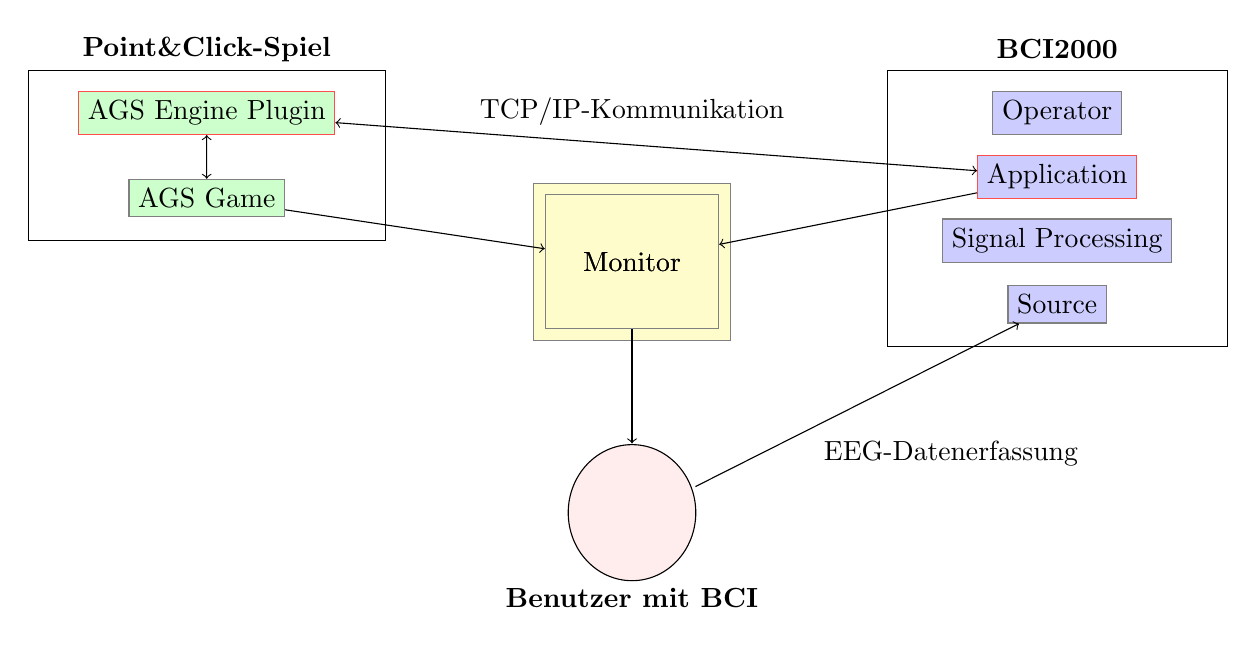
\begin{tikzpicture}[scale=1.08,
bci/.style={rectangle,draw=black!50,fill=blue!20},
bci2/.style={rectangle,draw=red!70,fill=blue!20},
game/.style={rectangle,draw=black!50,fill=green!20},
game2/.style={rectangle,draw=red!70,fill=green!20},
rechteck/.style={rectangle,draw=black!50,minimum height=17mm,minimum width=22mm},
display/.style={rectangle,draw=black!50,fill=yellow!20,minimum height=20mm,minimum width=25mm},
empty/.style={rectangle,draw=black!0,fill=black!0}]


% BCI2000
\def\X{5}
\node (bci2000) at (\X,0.75) {\textbf{BCI2000}};
\node[bci] (operator) at (\X,0) {Operator};
\node[bci2] (application) at (\X,-0.75) {Application};
\node[bci] (signal) at (\X,-1.5) {Signal Processing};
\node[bci] (source) at (\X,-2.25) {Source};
\draw (3,0.5) -- (7,0.5) -- (7,-2.75) -- (3,-2.75) -- (3,0.5);

\node at (0,0.02) {TCP/IP-Kommunikation};

% Point and Click Game
\def\X2{-5}
\node (game) at (\X2,0.75) {\textbf{Point\&Click-Spiel}};
\node[game2] (plugin) at (\X2,0) {AGS Engine Plugin};
\node[game] (game) at (\X2,-1) {AGS Game};
\draw (-2.9,0.5) -- (-7.1,0.5) -- (-7.1,-1.5) -- (-2.9,-1.5) -- (-2.9,0.5);

% Monitor
\node[display] (display) at (0,-1.75) {Monitor};
\node[rechteck] (display) at (0,-1.75) {Monitor};

% Subject
\node[empty] (subjectTop) at (0,-4) {};
\node[empty] (subjectRight) at (0.631,-4.45) {};
\draw[fill=pink!30] (0,-4.7) ellipse (0.75 and 0.8);
\node (userbci) at (0,-5.7) {\textbf{Benutzer mit BCI}};
\node at (3.75,-4.0) {EEG-Datenerfassung};

% Arrows
\draw [<->] (application) -- (plugin);
\draw [<->] (game) -- (plugin);
\draw [->] (game) -- (display);
\draw [->] (application) -- (display);
\draw [->] (display) -- (subjectTop);
\draw [->] (subjectRight) -- (source);

\end{tikzpicture}
\caption{Eine einfache Übersicht der einzelnen Bestandteile und deren Zusammenhänge. Die zu entwickelnden Kernkomponenten der BCI-Erweiterung sind mit einer roten Umrandung versehen.}
\label{Overview}
\end{center}
\end{figure}




\subsubsection{Die zu realisierenden Komponenten dieser Arbeit}
\begin{itemize}
\item Das Anwendungsmodul für BCI2000
\item Das AGS Engine Plugin, mit dessen Hilfe das Anwendungsmodul des \acs{BCI2000} mit dem Spiel kommunizieren und die Parameter austauschen kann.
\item Ein Point\&Click Spiel, welches die \acs{BCI}-Steuerung des AGS Engine Plugins verwendet und demonstriert.
\end{itemize}





\pagebreak
\section{Das BCI2000 Anwendungsmodul}

Dieses Kapitel behandelt die Definition, Auswahl und Planung des BCI2000 Anwendungsmoduls.

\subsection{Szenarien}
\vspace{0.3cm}
Im Zuge der Konzeption existierten zwei zu betrachtende Möglichkeiten, wie das Anwendungsmodul realisiert werden könnte.

\begin{itemize}
\setlength{\itemsep}{0pt}
\footnotesize
{
\item[1.] Implementierung der P300-Speller Funktionalitäten innerhalb des AGS Engine Plugins als sogenannte "`External Application"' des \acs{BCI2000}
\item[2.] Implementierung eines Anwendungsmoduls für die Verarbeitung von Speller-Matrix-Anfragen des \acs{AGS} Engine Plugins, basierend auf dem bestehenden P300 Speller des \acs{BCI2000}\\
}
\end{itemize}

\subsubsection{Szenario 1}
Das erste Szenario würde die Engine-Erweiterung und das BCI2000 Anwendungsmodul kombinieren. 
Dies würde mit sich bringen, dass sehr nah an der Engine gearbeitet wird und dortige Werkzeuge für die Visualisierung verwendet werden könnten.
Allerdings ist an dieser Stelle nicht bekannt, welche Möglichkeiten sich daraus ergeben und in wie weit diese limitiert sind, 
insbesondere da die Engine auf die Verwendung der Grafikbibliothek "`Allegro"' in der Version 4 begrenzt ist.
Bei der Untersuchung der \acs{BCI2000}-Plattform stellte sich jedoch heraus, 
dass die Architektur des bestehenden P300-Spellers und die Verknüpfung der Stimuli-Assoziationen zwischen P300-Speller 
und "`Source"'-Modul sehr komplex und besonders zeitkritische Faktoren sind.

\subsubsection{Szenario 2}
Die zweite Möglichkeit wäre die Entwicklung eines Anwendungsmoduls auf Basis des bestehenden P300-Spellers.
Auf diese Weise wären \acs{AGS} Engine Plugin und Anwendungsmodul zwei getrennte Komponenten, welche lediglich via TCP/IP miteinander kommunizieren.
Der daraus resultierende "`AGS-P300-Speller"' würde vor jeder Anfrage des Spiels die entsprechenden Parameter zugesendet bekommen. 
Die Größe, Position und der Typ der Speller-Matrix, sowie das aktuelle Bild des Spiel-Auschnitts würden alles abdecken, sodass der Speller darauf arbeiten könnte.
Hierbei würde im Hintergrund das Bild dargestellt werden und die Speller-Matrix würde auf dieses Bild überlagert werden, um die Eingaben zu ermitteln.
Diese Variante würde es theoretisch ermöglichen, dass zusätzliche Erweiterungen für andere Spiele Engines entwickelt werden könnten, welche auf die gleiche Weise mit dem Speller kommunizieren könnten.\\\\

\subsubsection{Auswahl des Szenarios}
Szenario 2 ist nach Abschluss der Recherche im Rahmen dieser Masterarbeit am sinnvollsten, da diese Variante basierend auf dem bestehenden P300-Speller auf ein funktionierendes Konzept aufbaut.
Denn durch eine potentielle Neuentwicklung des P300-Spellers besteht die große Gefahr, dass der "`AGS-P300-Speller"' nicht korrekt funktioniert.

Insbesondere müssen die Stimuli des Spellers mit den entsprechenden Signalen des "`Source"'-Moduls verknüpft werden.
Die Visualisierung der Stimuli und deren Assoziation spielt sich jedoch im Millisekunden-Bereich ab und ist somit generell zeitkritisch.\\

Eine Neuentwicklung und ein damit verbundener Mehraufwand zur Fehlerbehebung könnte möglicherweise den zeitlichen Rahmen dieser Masterarbeit übersteigen 
und ist demzufolge ein nicht kalkulierbares Risiko, das die Auswahl des 2. Szenarios begründet.\\







\pagebreak
\subsection{Konzept}

Das \acs{BCI2000} Anwendungsmodul kann für sich selbst in einem Aktivitätsdiagramm (siehe Abbildung \ref{aktivitaetsdiagrammbci2000}) dargestellt werden. 
Zunächst wird es zusammen mit der \acs{BCI2000}-Plattform gestartet und geht in eine Warteschleife über. 
In dieser Schleife wartet es auf eine Anfrage des AGS Engine Plugins oder einen Beenden-Befehl.
Sobald eine Anfrage erhalten wurde, werden die darin enthaltenen Parameter ausgewertet.
Aus den Parametern wird die Speller-Matrix aufgebaut und der aktuelle Bildausschnitt in den Hintergrund gelegt, so dass anschließend die Stimuli-Sequenzen vor diesem Hintergrund visualisiert werden.
Nach Abschluss dieser Prozedur wird das Ergebnis zurück an das AGS Engine Plugin gesendet und der Speller betritt bis zur nächsten Anfrage wieder die Wartschleife. \\\\




\begin{figure}[h!]
\begin{center}
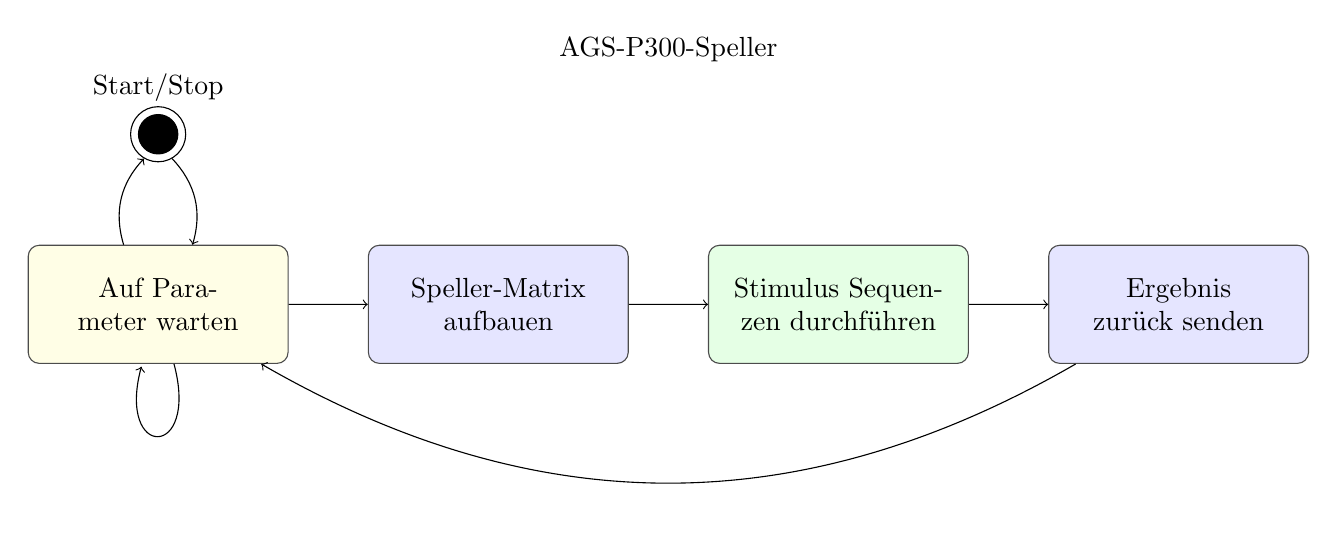
\begin{tikzpicture}[scale=1.08,
rect0/.style={line width=2pt,rectangle,draw=black!100,fill=red!10,minimum width=33mm,text width=30mm,minimum height=15mm,align=center, rounded corners},
rect1/.style={rectangle,draw=black!70,fill=blue!10,minimum width=33mm,text width=30mm,minimum height=15mm,align=center, rounded corners},
rect2/.style={rectangle,draw=black!70,fill=green!10,minimum width=33mm,text width=30mm,minimum height=15mm,align=center, rounded corners},
rect3/.style={rectangle,draw=black!70,fill=yellow!10,minimum width=33mm,text width=30mm,minimum height=15mm,align=center, rounded corners},
circle1/.style={circle,draw=black!100,fill=black!100,minimum width=5mm,minimum height=5mm,align=center},
circle2/.style={circle,draw=black!100,fill=black!0,minimum width=7mm,minimum height=7mm,align=center},
]

% BCI2000 Aktivitätsdiagramm
\node at (20mm, 0) {AGS-P300-Speller};

\node at (-40mm, -0.45) {Start/Stop};
\node[circle2] (start) at (-40mm, -1) {};
\node[circle1] at (-40mm, -1) {};
\node[rect3] (params) at (-40mm, -3) {Auf Para\-meter warten};
\node[rect1] (setup) at (0mm, -3) {Speller-Matrix aufbauen};
\node[rect2] (sequence) at (40mm, -3) {Stimulus Sequenzen durchführen};
\node[rect1] (result) at (80mm, -3) {Ergebnis zurück senden};

\path[->] 	(params) 	edge 					node {} (setup)
			(setup) 	edge 					node {} (sequence)
			(sequence) 	edge 					node {} (result)
			(result) 	edge 		 [bend left]node {} (params)
			(start) 	edge 		 [bend left]node {} (params)
			(params) 	edge 		 [bend left]node {} (start)
			(params)	edge 		[loop below]node {} (params);
			
\end{tikzpicture}
\caption{Das Aktivitätsdiagramm des AGS-P300-Spellers.}
\label{aktivitaetsdiagrammbci2000}
\end{center}
\end{figure}










\pagebreak
\section{Das \acs{AGS} Engine Plugin}
Da für das Anwendungsmodul Szenario 2 ausgewählt wurde, wird das AGS Engine Plugin lediglich die Verbindung herstellen 
und die Kommunikation zwischen dem Spiel und dem \acs{AGS}-P300-Speller übernehmen.
Dafür muss die Erweiterung Methoden bereitstellen, so dass Eingabe-Anfragen an den Speller gesendet werden können. 
Die Speller-Matrix Parameter sind zugleich auch die benötigten Parameter der entsprechenden Methode.
Lediglich den aktuellen Bildausschnitt holt sich das Plugin direkt von der Engine. 
Das Flussdiagramm des Spiels und des Plugins sind in Abbildung \ref{diagrammplugin} zu sehen. \\ \\


\begin{figure}[h!]
\begin{center}
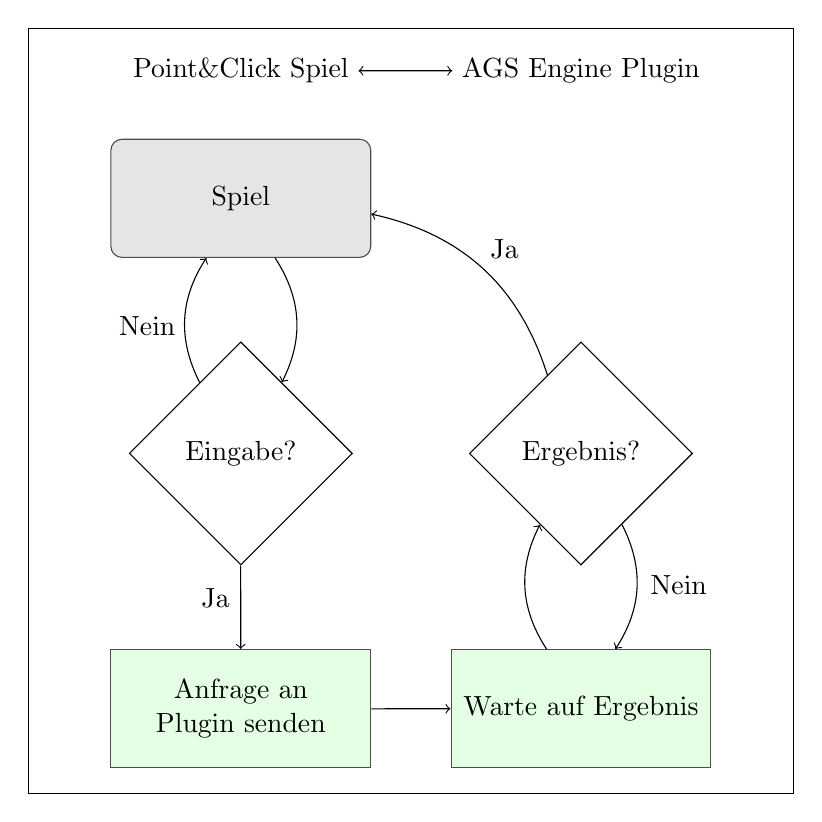
\begin{tikzpicture}[scale=1.08,
rect0/.style={line width=2pt,rectangle,draw=black!100,fill=red!10,minimum width=33mm,text width=30mm,minimum height=15mm,align=center, rounded corners},
rect2/.style={rectangle,draw=black!70,fill=green!10,minimum width=33mm,text width=30mm,minimum height=15mm,align=center},
rect3/.style={rectangle,draw=black!70,fill=black!10,minimum width=33mm,text width=30mm,minimum height=15mm,align=center, rounded corners},
raute/.style={rectangle,rotate=45,draw=black!100,fill=black!0,minimum width=20mm,minimum height=20mm, align=center}]

% AGS Engine Plugin Aktivitätsdiagramm

\draw (-6.5,0) -- (2.5,0) -- (2.5,-9) -- (-6.5,-9) -- (-6.5,0);
\node (a) at (-4, -0.5) {Point\&Click Spiel};
\node (b) at (0, -0.5) {AGS Engine Plugin};


%\node[rect3] (game) at (-4, -2) {};
\node[rect3] (game) at (-4, -2) {Spiel};

\node[raute] (check) at (-4, -5) {};
\node at (-4, -5) {Eingabe?};
\node at (-4.3, -6.7) {Ja};
\node at (-5.1, -3.5) {Nein};
\node[rect2] (control) at (-4, -8) {Anfrage an Plugin senden};

\node[rect2] (result) at (0, -8) {Warte auf Ergebnis};
\node[raute] (check2) at (0, -5) {};
\node at (-0, -5) {Ergebnis?};
\node at (1.15, -6.55) {Nein};
\node at (-0.9, -2.6) {Ja};

\draw [<->] (a) -- (b);

\path[->]	 (game)		edge 	     [bend left]node {} (check)
			 (check)	edge 	     [bend left]node {} (game)
			 (check)	edge 					node {} (control)
			 (control)	edge 					node {} (result)
			 (result)	edge 		[bend left] node {} (check2)		
			 (check2)	edge 		[bend left] node {} (result)			
			 (check2)	edge 		[bend right] node {} (game);
			
\end{tikzpicture}
\caption{Das Flussdiagramm zwischen Spiel und AGS-P300-Speller Plugin}
\label{diagrammplugin}
\end{center}
\end{figure}




\pagebreak
\section{Point\&Click Test-Spiel}

Im Anschluss an die Implementierung der BCI-Erweiterung wird in diesem Abschnitt ein einfaches Test-Spiel konzipiert.
Dieses Spiel soll im späteren Verlauf für Tests verwendet werden, so dass Ergebnisse gesammelt und ausgewertet werden können.\\

Das Test-Spiel soll ein kurzes und einfaches Szenario darstellen, so dass die späteren Testpersonen lediglich einige Eingaben durchführen müssen um eine Aufgabe zu erfüllen.
Das Szenario wird gemäß des Titels dieser Masterarbeit an "`The Secret of Monkey Island"' angelehnt sein und sich daher optisch in diese Richtung orientieren.
Die Aufgabe wird es sein einen fiktiven Charakter über einen Strand laufen zu lassen und mit anderen Charakteren zu reden oder Gegenstände aufzuheben, 
um diese an einen Zielort zu bringen. 
Die Eingabe würde über einen P300-Speller erfolgen.\\

In Abbildung \ref{gameconcept} ist eine Skizze zu sehen, wie die Spielszene aussehen könnte.
Ein Befehl an die Spielfigur würde dann so ablaufen, dass zunächst mit dem Speller ein Befehl in der unteren GUI-Leiste ausgewählt und anschließend ein Ziel für diesen Befehl ermittelt wird.
Je nach ausgewählten Befehl kann sich die Position der Speller-Matrix entsprechend an die Position der möglichen Ziele anpassen.
Da die Speller-Matrix eine gewisse Mindestgröße benötigt, kann es hier durchaus nötig sein, dass eine Schaltfläche für einen Befehl durch mehrere Zeilen und Spalten abgedeckt werden muss.


\begin{figure}[h!]
\begin{center}
\includegraphics[scale=0.3]{images/szene1konzept.png}
\caption{Skizze einer Szene mit Speller-Matrix des Typs 5x8 inkl. blau hervorgehobener Zeile (Stimuli)}
\label{gameconcept}
\end{center}
\end{figure}









































